Big Data has transformed our society in the last years. The capability to develop efficient applications which were able to handle large amount of data at run time was the first step. In section \nameref{Data-Intensive Applications}, first of all, a classification of these kind of application is made. After that, the characteristics of data-intensive applications are explained. Finally, in this section some frameworks as Hadoop, Spark or Flink are explained giving some characteristics and what makes them different. In section \nameref{Privacy Policies in IT} some concepts relative to computer security and how such concepts impact on data privacy are developed. Some different approaches to generate private data are exposed and, after that, it is emphasized how privacy policies can be applied in the already known data-intensive applications. Finally, in section \nameref{Modeling and Metamodeling}, first of all the main concepts of metamodeling are exposed. After that the Unified Model Language is explained and, at the end of the section, a model-driven approach to support data-intensive application design called StreamGen is introduced.

\section{Data-Intensive Applications}

\label{Data-Intensive Applications}

Data-Intensive Applications (DIAs), according to \cite{cloudcomputing}, are a class of parallel computing applications which handle high amount of datasets and that devote the most of their processing time to I/O and manipulate such datasets. These kind of applications are able to manage datasets of several terabytes and petabytes which are available in a wide variety of formats and that are distributed among several locations. This capability to process large volumes of data is possible due to the fact that DIAs use multi-step analytical pipelines with transformations and fusion stages in order to parallelize the execution of the data.

Intensive applications can be classified (\cite{parallelcomputing}, \cite{computing21} and \cite{dataintensivecomputing}) according to the parallel processing approaches commonly known as compute-intensive and data-intensive. On the one hand, compute-intensive is used to describe application programs that are compute bound. Such applications devote most of their execution time to computational requirements and they process small volumes of data. In this kind of applications, processes must be parallelized by means of individual algorithms and then they must be decomposed into separate tasks. Later, such tasks are executed in a pipeline reaching higher performance that in serial processing. Finally, compute-intensive applications are able to perform multiple operations simultaneously as they allow task parallelism.

On the other hand, data-intensive is used to describe application programs that are I/O bound (\cite{dataintensivecomputingIEEE}). Such applications devote most of their execution time to I/O, move and manipulate the datasets. This second parallel processing approach, unlike compute-intensive, processes large volumes of data. Data-intensive applications require the partition or subdivision of the initial dataset in some smaller datasets due to the fact that the large volume of data that they are composed. These partitions must be processed independently by the application allowing the parallelization of the initial dataset. Once the partitions are executed, they must be reassembled in an output dataset.

As any type of application which takes advantage of data-parallelism, DIAs need to select an algorithm not only to distribute data among the processing nodes of the cluster but also to execute the data in such processing nodes (\cite{terascalechallenge}). Moreover, they need to adopt a strategy to decompose the datasets, find a trade-off in terms of working loads in the processing nodes by means of load balancing systems and to communicate the nodes of the cluster.

\subsection{Characteristics}

Data-intensive applications are modeled in a different way than any other computing application due to the property of DIAs to be processed in a cluster infrastructure. Moreover, as any other system, DIAs need to reach a high performance in order to make efficient applications; this is possible by means of the minimization of the number of movements of the data. Other important properties required by DIAs are that they must be available when they are called, and that they must be reliable to the number of failures; both properties are accomplished due to data-intensive applications are fault resilient. Last but not least, data-intensive applications must be able to change the number of required nodes taking into account the workload. Then, four characteristics, according to \cite{distributedcomputing} and \cite{scalablecomputing}, can be defined in order to distinguish data-intensive applications from any other kind of computing system:

\subsubsection*{Dataflow Model}

Data-intensive applications are modeled by means of nodes where some transformations take place and data or programs flow between such nodes. Moreover, such model allows to control how to schedule, to execute, to balance the load and to communicate programs and data during runtime using a cluster computing infrastructure.

\subsubsection*{Data Movement Minimization}

Minimize the number of movements required by each data along the different computations in order to achieve high performance is crucial in data-intensive applications. Then, processing algorithms are executed on the nodes of the dataflow model where the data is located, reducing the number of movements and therefore increasing performance.

\subsubsection*{Fault Resilient}

Due to the fact that DIAs work with high amounts of data, the probability for the hardware to fail is greater than in other computing systems but the same happens with the probability of communications errors and software bugs. This is why, DIAs are designed to be fault resilient. In order to make these applications available and reliable, on the storage disk of such systems redundant copies of all data files or intermediate processing results can be found. But also they are provided with systems capable to detect the failure of any node or processing failures and, once such failures are detected, then re-compute the results.

\subsubsection*{Node Variability}

Depending on the hardware and software architecture of the data-intensive application, the required number of nodes and processing tasks and its variability along the runtime can be fix or variable. This is due to the fact that it is very important to achieve a comfortable processing independently of the amount of data and, also, to reduce the critical time of computation by adding some nodes.

\subsection{Frameworks}
\subsubsection{Apache Hadoop}

Apache Hadoop is an open source software framework that supports distributed applications. As any other DIA, Hadoop allows to work with thousands of nodes and petabytes of data. This framework is composed by a processing layer called MapReduce which was inspired by Google documentation.

MapReduce works as a DIA processing large volumes of data. First of all, this programming model divides the incoming works into a set of independent tasks and, after that, such tasks are executed. Then, the user sends the complete job to a master which divides it into independent tasks and submits them to the slaves in order to process the works in parallel. This process allows Hadoop to reach speed and reliability of cluster.

In summary, Hadoop MapReduce works breaking the incoming datasets into independent sets that are executed in parallel by means of two phases (\cite{hadoopwebsite}): map phase and reduce phase. Firstly, in the map phase, the business logic is specified by putting the custom code in the way MapReduce works. And, secondly, in the reduce phase, operations as summations and aggregations are processed.

\subsubsection{Spark}

Spark is an open source platform that allows general-purpose and fast cluster computing. It is an engine that allows to process large volumes of data.

Spark enables users to access repeatedly to datasets in order to perform streaming, machine learning or SQL workloads by means of high-level APIs in Java, Scala, Python and R. It also allows users to accomplish batch processing or stream processing.

Moreover, Spark can be integrated with any other data-intensive tool due to its design. Spark is compatible with Hadoop as it is able to access Hadoop data sources and run on Hadoop clusters. This platform extends MapReduce, the engine of Hadoop, by including iterative queries and stream processing.

Some features make Spark more efficient than Hadoop. The following features, that are presented in \cite{sparkwebsite}, make Spark being the 3G of Big Data:

\begin{itemize}

\item Fault tolerance.
\item Dynamic in nature.
\item Reusability.
\item Advanced analytics.
\item Lazy evaluation.
\item Real-time stream processing.
\item In-memory computing.

\end{itemize}

The in memory computing feature reduces the number of read-write to disk operations what achieves a data processing performance 100 times faster in memory and 10 times faster on the disk. Due to the high amount of operators that Spark provides, to achieve parallel applications is easier with Spark. Regarding to fault tolerance, Sparks handles the failure of the nodes in the cluster by means of Resilient Distributed Datasets (RDDs) which its specific design makes to reduce the number of failures to zero.

In conclusion, Spark can be differentiated from Hadoop in its cluster management system. On the other hand, regarding to the similarities between Spark and Hadoop, Spark takes advantage of Hadoop for storage.

\subsubsection{Apache Flink}

Apache Flink is an open source platform which allows data streaming computation because of its data flow engine. According to \cite{streamprocessing}, data stream processing is to compute on data just when it is received or produced. Moreover, as happens with Spark, Apache Flink is able to execute stream processing and batch processing and it is also compatible with Hadoop.

Apache Flink can undertake efficiently some different types of processing, becoming in the most potent open source platform in the market to handle them. Such processing types, according to \cite{flinkwebsite}, are:

\begin{itemize}

\item Batch Processing.
\item Interactive processing.
\item Real-time stream processing.
\item Graph Processing.
\item Iterative Processing.
\item In-memory processing.

\end{itemize}

Apache Flink reduces the complexity that other platforms as Spark faced by means of some improvements. Such improvements include the integration of query optimization in MapReduce processing layer, some concepts from database systems and efficient parallel in-memory and out-of-core algorithms. These optimizations are given due to the fact that Flink architecture is designed taking into account the streaming model. Such design improves the micro-batch approach taken in Spark for data streaming processing making Flink faster and with lower latency for such kind of processing.

Following the example of Spark, Apache Flink is provided with three APIs (DataStream, DataSet and Table APIs) in order to use its engine. DataStream and DataSet APIs are two regular programs used by Flink in order to perform transformations on data streams (filtering, aggregating, update state...) and data sets (joining, grouping, mapping...) respectively. On the other hand Table API is used for relational operations and it can be integrated into DataStream API for relational stream processing and into DataSet API for relational batch processing.

Finally, it is important to remark the five features that can be found in \cite{flinkwebsite} about Apacha Flink:

\begin{enumerate}

\item Low latency and high performance.
\item Fault tolerance.
\item Memory management.
\item Iterations.
\item Integration.

\end{enumerate}

All these characteristics are what make Flink the 4G of big data and the most powerful tool when dealing with data stream processing.

\section{Privacy Policies in IT}

\label{Privacy Policies in IT}

The appearance of Big Data and DIA platforms dealing with large amount of datasets has led the society to question about the privacy of those data that are processed. Due to the fact that such data are not visible for the data producers but these data are bought and handled by many companies in order to compute some statistics, data privacy has become in a must for the development and commercialization of new DIA in order to give the option to the user to decide on which data can be seen by other agents.

On the other hand, large amount of data flowing through the net and the existence of black hat hackers forces DIA designers to take into account some concepts about computer security (\cite{computersecurityslides}). Computer security, also known as cybersecurity or information technology security (IT security), is the protection of computer systems and networks from people who is interested in stealing or damaging their hardware, software or the data with which they are working. It is at this last point where Big Data applications have to pay attention in order to be designed.

Every computer security system accomplish the well-known CIA paradigm, as it is explained in \cite{computersecurityslides}. "C" stands for Confidentiality, "I" for Integrity and "A" for Availability and they are the three basic requirements that compose such paradigm. Any computer security system has to grant that any piece of data has to be accessed only by those who are authorized, accomplishing such requirement, information is confidential. Moreover, such systems have to be able to allow data modifications only to those how are authorized for it and only in the way that they are entitled to modify them, this requirement makes information to be integrated. Finally, data must be available to everyone who has a right over them within some time constraints, this makes information to be available. These three requirements raise an engineering problem and it is that availability conflicts with confidentiality and integrity due to the fact that if a data is available then it could not be confidential as anybody may modify it and it could not be integrated as anybody could modify then. This is the main problem that has to be faced when designing computer security problems. In order to handle this complex engineering problem, designers can use legal instruments but also technical tools.

Due to the fact that the information of many entities (persons, companies, etc.) are involve in such complex problem, there are some legal instruments to handle the design of security systems. This is the case of privacy policies. Privacy policies are statements or legal documents that reveal how an entity can collect, use or handle data from another entity. Privacy policies can differ from one country to another this is why there are some agreements in order to handle them. In the European Union (EU) the General Data Protection Regulation (GDPR), according to its web page \cite{gdprwebpage}, is in charge of harmonizing data privacy laws across all member states of the EU. In spite of these regulations, there are many ways in order to apply privacy policies.

Due to the importance of such privacy policies, some researchers haven been studying about the development of formal languages in order to specify them in a logical way. This is the case of some literature \cite{XACMLlanguage} where XACML is used to specify privacy policies by means of some logic rules in order to reach a set of policies. This formal language (XACML) also can be used for other reasons as it is the case of user authentication in distributed systems \cite{XACMLforAuthentication}.

On the other hand, when a computer security system is designed, the designer has to put himself in the place of the cyberthief, or threat agent, in order to achieve a secure system. Such cyberthieves try to find vulnerabilities and, then, exploit them in order to steal some information. Usually, vulnerabilities are a bug that allows to violate the CIA paradigm but the exploit can be a wide variety of vulnerability uses. Despite this design technique, unfortunately, a great amount of vulnerabilities are found when users accidentally deal with the applications once the applications are in the market.

Another remarkable point is the importance of threats, that are potential violations of the CIA paradigm in computer security systems. This means that an information system can be seen its security system broken due to the fact that a circumstance or an event could impact on it adversely by means of the break of any of the three basic requirements of a computer security system. A threat is composed by three layers. The attacker or threat agent that is the person or the information system that performs the attack action, the countermeasure layer that is all the systems that try to identify an attack and to stop it and, finally, the target of the attack that is on which resides the vulnerability and on the threat consequences take place when the exploit arrives to the vulnerability. By means  of such vulnerabilities, private data can be stolen by cyberthieves. This is why, system dealing with confidential data must hash them as soon as possible in order to handle private data even during the execution phase of the pipeline.

In conclusion, the concept of computer security involves many fields but when dealing with the design of DIAs, it is very important to take into account not only the CIA paradigm but also the design techniques from the threat agent perspective in order to reach secure DIAs, always under the legal framework of privacy policies. Furthermore, what makes security on DIAs reliable is the balance on its conflicting requirements what is a complex engineering problem. Finally, systems with a high amount of vulnerabilities but with no threats, are secure systems. However, systems with many threats and only a few vulnerabilities become in the most attacked systems and, then, the ones that need more security measures.

\subsection{Privacy Policies in DIAs}

Due to the fact that DIAs are constantly managing data from different entities, it is very important the way in which privacy policies are applied on them. The final goal of applying them is that, in case of threats, threat agents cannot obtain such data. This reduces the probability of threats as there is no sensitive data that can be obtained and, then, the CIA paradigm cannot be broken.

When dealing with DIAs, sensitive data are sent in data streams. Such data streams are composed of tuples which can contain a high variety of data. Each tuple of a data stream contains a finite set of data that are always ordered in the same way. Due to the fact that all the tuples contained in a data stream have the same structure, when speaking about data streams, each of the data of the tuple is considered as a field of the data stream. Due to this distinction on the fields of the data streams, some literature \cite{privacypoliciesarticle} classifies data streams into three different sets:

\begin{itemize}

\item Subject-specific streams.
\item Subject-generic streams.
\item Non-personal streams.

\end{itemize}

A subject-specific stream is a stream composed of a field referring to the data subject. This means that each tuple of the stream contains a data which is the owner of the tuple. A subject-generic stream is a stream without data subject. However, subject-generic streams are produced by an operator whose input is a subject-specific stream. Finally, a non-personal stream is a stream without data subject and that it has not been produced by an operator whose input is a subject-specific stream.

The context in which a tuple is conveyed is also important. Depending of the context in which data are transferred, an entity could want that the data of the tuple are private or public. This context is specified by means of three variables in \cite{privacypoliciesarticle}:

\begin{itemize}

\item Observer.
\item Role.
\item Purpose.

\end{itemize}

The first variable is the observer of the data, the entity who demands the usability of the data. The second variable is the role that the requesting entity is playing. The requesting entity can be a person but also a company. In the case of the company, many persons working for such company can be demanding the data of the tuple and each person has a role inside the company, this is why the role is an important variable in order to define the context in which a privacy policy can be applied. Finally, the third variable that defines the context is the purpose. The purpose for which the requesting entity demands the data of the tuple. Then, the context in which a privacy policy has to be applied is defined by means of three variables that are called static context variables (SCV) as, once they are defined, they are not going to change and because of this they are static.

Another important distinction is the one given by the data that compose a tuple. Each of these data can be strings or numbers. Because of this, a classification on the type of each data of the tuple, and then on the type of the fields of the streams, has to be defined. Moreover, following the approach given by the SCVs, each of these values are considered as a variable as the values of a field of a given stream can change depending on the tuple that is referred. Then, the variables that compose a field of a stream, according to \cite{privacypoliciesarticle}, are:

\begin{itemize}

\item Categorical variables.
\item Numerical variables.

\end{itemize}

Categorical variables are those that correspond to a string in any programming language. They can be words but also links or any set of letters with special characters and numbers. The second type of variables correspond to numbers but also to a range which corresponds to a pair of numbers. For example, a data subject can be a categorical variable when it is the name of the user who uses the DIA but a data subject can be also a numerical variable if it is an ID which is compose only by numbers. Furthermore, the set of categorical and numerical variables used by a DIA are called contextual variables.

Taking into account these three classifications, privacy policies can be defined by means of some rules. These rules have to be defined making a relationship between the contextual variable used by the DIA and some values that the user selects in order to encrypt the original fields of the stream. These relationships are made by means of logical operators. In the case of categorical variables, the operators that can be used are: equal to ($=$) and not equal to ($\neq$). On the other hand, in the case of numerical variables, the relation operators that can be used are: equal to ($=$), not equal to ($\neq$), is greater than ($>$), is less than ($<$), is greater than or equal to ($\geq$) and is less than or equal to ($\leq$)

Finally, due to the fact that privacy policies encourage the anonymity of the entity who owns the data of the tuple, depending on the data stream classification explained above and the rules defined by each user, privacy policies can differ. Then, another classification is made in \cite{privacypoliciesarticle}, in this case about the privacy policies in DIAs:

\begin{itemize}

\item View Creation Policies (VCPs).
\item Data Subject Eviction Policies (DSEPs).

\end{itemize}

\subsubsection{View Creation Policies (VCPs)}

View Creation Policies (VCPs) are a type of privacy policies for DIAs which are applied to subject-specific streams. VCPs are applied when the context is precisely specified by means of the SCVs and the information contained in all the fields of the stream is observable, which means that it has not been modified before by another privacy policy.

Furthermore, VCPs are defined by means of a set of rules which are relationships between the contextual variables used by the DIA and some values that the user selects in order to encrypt the original fields of the stream. In this kind of privacy policies, the encrypted final values of the stream are defined by means of generalization vectors. A generalization vector defines the value to be used in order to generalize each of the fields that compose a subject-specific stream.

In conclusion, given a tuple belonging to a subject-specific stream, if at any instant such tuple satisfies all the rules defined by means of logical operators relating some contextual variables with a value defined by the user of the DIA, a generalization vector is applied on the tuple in order to generalize each of the fields of the streams and obtaining an encrypted tuple. Then in \cite{privacypoliciesarticle}, a VCP is defined by means of four items:

\begin{enumerate}

\item Subject-specific stream.
\item Data subject.
\item Set of relational rules.
\item Generalization vector.

\end{enumerate}

\subsubsection{Data Subject Eviction Policies (DSEPs)}

Data Subject Eviction Policies (DSEPs) are applied when given an operator, which input is a subject-specific stream, produces a subject-generic stream. Sometimes, the entity who owns the data which are flowing along the DIA does not want that an operator takes some information from the input stream in spite of the output stream is not showing any information directly pointing to such owner. This is the case in which DSEPs are applied.

Unlike what happens with VCPs, DSEPs do not encrypt the fields of a given data stream. In this case, DSEPs prevent the tuples flowing in the subject-specific stream that inputs into a given operator from being processed by such operator. In this case, the output from the operator is computed without taking into account the data of the data subject who defines the DSEP, preserving the anonymity of the owner of the data for the computation of a certain statistic.

In conclusion, in order to define a DSEP, first of all, a set of rules have to be specified by the user relating some contextual variables with some values that such user has to define. Then, given an instant when all the defined rules are satisfied on a subject-generic stream which outputs from a given operator, all the tuples referring to the data subject who defined such rules have to be evicted from the subject-specific stream that inputs into the given operator. Then in \cite{privacypoliciesarticle}, a DSEP is defined by means of three items:

\begin{enumerate}

\item Subject-generic stream.
\item Data subject.
\item Set of relational rules.

\end{enumerate}

\section{Modeling \& Metamodeling}

\label{Modeling and Metamodeling}

Data Intensive Applications are used when large amount of data have to be handle with high performance. In order to reach such high performance, DIAs require complex designs and a lot of resources to achieve their goal. One of these resources is the number of software developers who are needed to write the application codes. On the other hand, when some specific requirements are added to the DIAs, as it is the case of privacy policies managing the privacy of the users, developing DIAs becomes in a really difficult task which cannot be faced writing codes from scratch. At this point is where other approaches to write application codes take advantage. Such is the case of modeling and metamodeling techniques applied to software development.

A model is a representation of a reality in order to explore, to redesign or to transform it. This representation can be externalized by means of a diagram in a paper or in a computer software. Modeling is the method that has to be developed in order to reach a model. A modeling method consists of a modeling technique and a mechanism or algorithm working on the model. Moreover, a modeling techniques consists of a modeling language and a modeling procedure. A modeling procedure is a sequential process composed of several steps but also an iterative process since the procedure can be repeated many times until the final model is reached. In spite of several modeling procedures can be accomplish in order to create a model, as it can be found in \cite{modelwebsite}, all these approaches share some common steps:

\begin{itemize}

\item Purpose definition.
\item Boundaries definition.
\item Model elements definition.
\item Relationships definition.

\end{itemize}

The first step that has to be accomplished in order to create a model is to define its purpose. With such purpose, the questions that the model will have to answer, once it is implemented, should be specified. Later, the boundaries of the model must be specified. Such boundaries must focus on the reality that has to be modeled discarding any information that is not able to reach the predefined purpose. Once these boundaries are defined, everything that is going to take part of the model is called the model domain. Due to the fact that usually this domain is still very big, each concept belonging to the model domain must be filtered taking into account the relevance of each of them and grouping those concepts that are identical in order to reach the purpose. After that, each of the groups with identical concepts can be transformed into a model element, which is an abstraction of all the concepts that are part of the group. Finally, the relevant relationships among the model elements have to be identified and represented in the model.

Furthermore, a model must be complete in order to be able to answer the question specified in the purpose but also, it must be consistent which entails the lack of contradictions in its representation. In order to reach such characteristics, modeling methods take advantage of modeling techniques in addition to a mechanism, an algorithm, working on the model.

The first component of a modeling technique that is a modeling language is a set of well-known elements and relationships by means of which a model can be represented. A modeling languages is described by a syntax, semantics and a formal notation. A syntax is the set of elements, relationships and rules that can be written in order to represent a model by means of a grammar. Moreover, a syntax can be described by two different types of grammars: graph grammars and metamodels. According to \cite{metamodelwebsite}, a metamodel is a model of a modeling language. A metamodel is written by means of a modeling language that is known as the metamodeling language. The metamodeling language has a model which defines it. This is why exists a modeling hierarchy which is not limited and that ends given a useful abstraction level of the model. In the table \ref{Modeling Hierarchy} there is an example of a modeling hierarchy with five levels.

\begin{table}[h!]
\centering
	\begin{tabular}{||c|c|c||} 
	\hline\hline
	Language Level & Models & Language Name \\ [1ex] 
	\hline\hline
	Level 1 & Model & Modeling Language  \\
	\hline
	Level 2 & Metamodel & Metamodeling Language  \\
	\hline
	Level 3 & $Meta^2$-Model & $Meta^2$-Modeling Language  \\
	\hline
	Level 4 & $Meta^3$-Model & $Meta^3$-Modeling Language  \\
	\hline
	Level 5 & $Meta^4$-Model & $Meta^4$-Modeling Language  \\
	\hline\hline
	\end{tabular}
\caption{Modeling Hierarchy}
\label{Modeling Hierarchy}
\end{table}

The semantics of a modeling language describe the meaning of the language by means of a semantic domain and a semantic mapping.

Finally, the formal notation describes how the modeling language is visualized. Some symbols are used in order to represent the represent the syntax of the language in a diagram.

On the other hand, the finality of the mechanism is to check that the model written with the modeling language by means of the modeling method is correct and satisfies the purpose of the model. There are three main types of mechanisms and algorithms: generic, specific and hybrid.

In the figure \ref{fig:Modeling Method Components} o model of a modeling method is shown.

\begin{figure}
\centering
{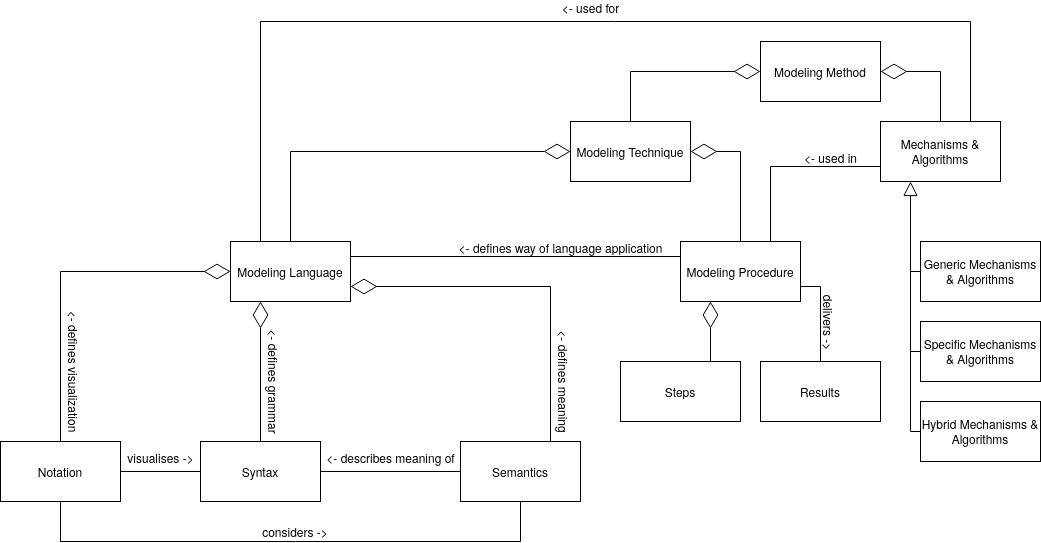
\includegraphics[scale=0.3]{./chapter2/compModelMethod.png}}
\caption{Modeling Method Components}
\label{fig:Modeling Method Components}
\end{figure}

\subsection{Unified Modeling Language (UML)}

Unified Modeling Language (UML) is a standardized modeling language whose objective is to provide system architects, software engineers, and software developers with tools for analysis, design, and implementation of software-based systems as well as for modeling business and similar processes.

UML is able to achieve such goal by means of a wide variety of options to build modeling diagrams. Among the fourteen possibilities that UML provides to construct a diagram, a distinction between two main classes is made in \cite{umlwebsite}: behavior diagrams and structural diagrams.

Behavior diagrams represent the dynamics of a system, this means the representation of all the possible changes that a system can experience over time. This class is composed of seven diagrams: activity diagram, communication diagram, interaction overview diagram, sequence diagram, state machine diagram, timing diagram and use case diagram.

On the other hand, structural diagrams represent the different static parts of the system, that ones which do not change over time. This representation can be done from different abstraction and implementation levels and making the corresponding relationships between the parts of the system. This second class is composed of other seven possibilities for diagram construction: class diagram, component diagram, component structure diagram, deployment diagram, object diagram, package diagram and profile diagram.

A UML diagram making a description of all the UML diagrams can be seen in the figure \ref{fig:UML Metamodel}.

\begin{figure}
\centering
{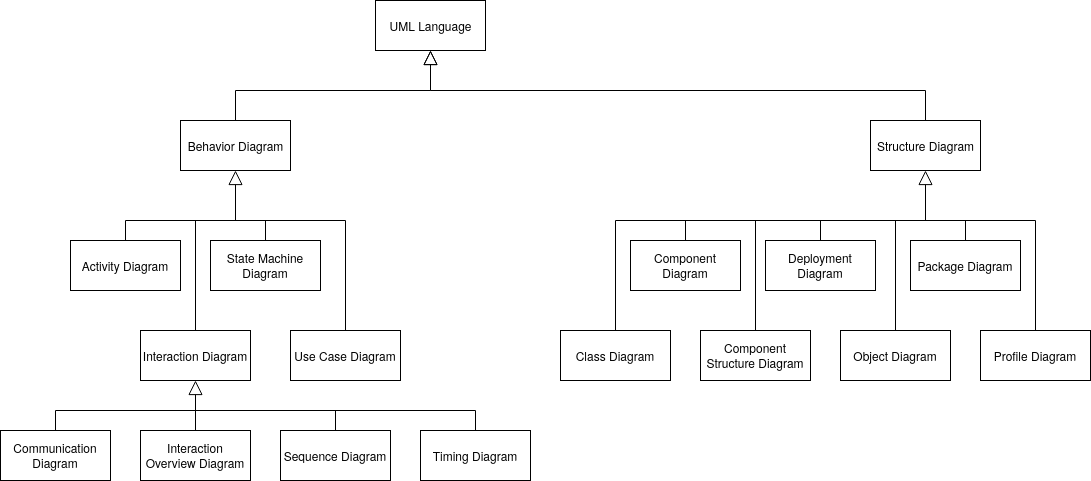
\includegraphics[scale=0.3]{./chapter2/umlMetamodel.png}}
\caption{UML Metamodel}
\label{fig:UML Metamodel}
\end{figure}

\subsubsection{UML Diagrams}

In spite of UML allows developers to use fourteen diagrams for modeling, some of such diagrams are the most commonly used. According to \cite{umlwebsite}, this is the case of the following ones:

\subsubsection*{Class Diagram}

This kind of diagram represents the model elements and the relationships that exist between such elements. The model elements, which are represented by means of nodes, can be: class, component, data type, interface, model or package among others. Regarding to the relationships between the nodes, they can be: association, association class, dependency, generalization or information flow among others.

Class diagrams are commonly used to represent the metamodel of the syntax of a modeling languages. Due to the fact that this kind of diagrams is not able to fully express syntactical rules, usually they take advantage of constraint languages as Object Constraint Language (OCL).

\subsubsection*{Profile Diagram}

A profile diagram allows to create the model domain by adding model elements called stereotypes and making the corresponding relationships between them. The most commonly used relationships in this kind of diagrams are the composition and the generalization.

\subsubsection{UML Frameworks}

Due to the UML popularity among software developers, there are several frameworks working with it in order to make software development easier. Different platforms can be used for UML modeling but also platforms for converting a model to a source code can be found.

\subsubsection*{Papyrus}

UML can be found in a wide amalgam of platforms due to its utility for modeling. Moreever, there are some platforms that are the most commonly used for software development. This is the case of Eclipse.  Eclipse is the most popular Java Integrated Development Environment which allows a large amount of plugins in order to increase its functionalities.

One of the plugins provided by Eclipse is Papyrus, an open-source UML tool. In spite of Papyrus was developed by the French Alternative Energies and Atomic Energy Commission (CEA-List), currently it is one of the most used UML tools for software development as it can be expanded with UML profile diagrams giving a wide functionality for modeling software applications.

\subsubsection*{Acceleo}

Regarding to platforms for converting an UML model into source code, Acceleo is an open-source generator from Eclipse Foundation. Acceleo is
one of the Eclipse plugins that allows to transform UML models into source code files. It is written in Java and it is available for Linux, Windows and Mac OS.

Acceleo uses its own language in order to generate the source codes. Such language is based on MOF Model to Text Transformation Language (MOFM2T) and on template focusing. A template contains some text which describes the data that should be extracted from the elements of the model and such data are extracted iteratively from each component of the model. Moreover, the descriptions of the information that should be taken from the model elements are written in OCL language.

Finally, it is import to remark that Acceleo can extract the information from different types of models, such as EMF, UML or DSL and it is able to generate different source languages such as C, Java or Python.

\subsection{Object Constraint Language (OCL)}

Object Constraint Language (OCL) is a language to describe formal expressions in UML models. These expressions represent invariants, preconditions, postconditions, initializations, guards, derivation rules, as well as queries to objects in order to determine its state conditions. 

Initially, OCL was developed by IBM. But, then, in 2003, OCL was adopted as part of UML 2.0 by the group OMG.

This language does not cause side effects, so the verification of a condition, which presupposes an instantaneous operation, never alters the objects of the model. Its main role is to complete the different artifacts of the UML notation with formally expressed requirements.

In conclusion, OCL associates boolean expressions with the elements of the model and these expressions are evaluated as true every time the program is executed. In addition, they can also be associated with methods. In this case, the Boolean expressions are evaluated as true at the moment before or after the execution of the program.

\subsection{StreamGen}
StreamGen is a model-driven approach to support the design of DIAs and the automated code generation for two target platforms, Flink and Spark. This approach is developed focusing on two requirements:

\begin{itemize}
\item To provide a platform-independent and graphical modeling language for streaming applications.
\item To enable the fast prototyping of distributed streaming applications over different platforms.
\end{itemize}

The first requirement is needed in order to develop any kind of DIA for different target platforms and, independently for which platform it is targeted, provide a complete language for all of them. This is possible due to the DIA dataflow model characteristic that supports the development of them by means of sources, transformations and sinks. The second requirement is satisfied by using UML class diagrams for such purpose. This kind of diagrams allow to represent sources, transformations and sinks but also the data flows really fast, just introducing the predefined stereotypes.

\subsubsection{DIA Generation Process}

The different steps that have to be followed in order to generate a DIA with StreamGen are the following:

\begin{itemize}
\item UML model creation.
\item Application code generation.
\item Application execution.
\end{itemize}

\subsubsection*{UML model creation}

First of all, the user must create a UML model by exploiting a predefined language in a UML profile diagram. This language consists of four metaclasses:

\begin{itemize}
\item Class
\item InformationFlow
\item Model
\item Package
\end{itemize}

The class metaclass represents the streaming operators stereotypes which are data sources, data sinks and data stream transformation. Moreover, this three stereotypes can be represented by means of several generalization. In the table \ref{StreamGen Classes} can be shown such stereotypes.

\begin{table}[h!]
\centering
	\begin{tabular}{||c|c|c||} 
	\hline\hline
	Sources & Transformations & Sinks \\ 
	\hline\hline
	Text File & Reduce & Text File \\ 
	\hline
	Socket & Map & CSV File \\ 
	\hline
	Collection & Window & Socket \\ 
	\hline
	Kafka & Flatmap & Cassandra \\ 
	\hline
	 - & NFlatmap & Kafka \\
	\hline
	 - & NMap & - \\
	\hline
	 - & Count & - \\
	\hline
	 - & Fold & - \\
	\hline
	 - & Sum & - \\
	\hline
	 - & Filter & - \\
	\hline
	 - & Join & - \\
	\hline
	 - & CoGroup & - \\
	\hline\hline
	\end{tabular}
\caption{StreamGen Classes}
\label{StreamGen Classes}
\end{table}

The InformationFlow metaclass represents the data streams. There are three main data streams stereotypes: non-parallel stream, windowed stream and partitioned stream. Moreover, the partitioned stream stereotype can be generalized to broadcasted stream, keyed stream, randomly partitioned stream and round robin stream.

The model metaclass is extended by a distributed streaming application stereotype which is generalized to Flink application, Spark application and Apex application.

The last metaclass, the package, is extended by the stream data types stereotype which will contain all the data types conveyed by the different information flows.

\subsubsection*{Application code generation}

Once the user has defined the UML model, the java application configuration must be run in order to generate the application codes. This is possible because of the development of an Acceleo code. This Acceleo program is able to take as inputs the generated UML model and, depending on the different stereotypes contained in such model, generate a DIA code for Flink or Spark.

\subsubsection*{Application execution}

Currently, StreamGen allows code generation for Spark and Flink. As can be seen in its model stereotypes, also there is an intention to develop Apex codes in the future.















